\documentclass[a4paper]{article}
\usepackage[fontsize=13pt]{scrextend}
\usepackage[utf8]{vietnam}
\usepackage{amsmath}
\usepackage{amsfonts}
\usepackage{xcolor}
\usepackage{titlesec}
\usepackage{mdframed}
\usepackage{amssymb}
\usepackage{pgf,tikz,pgfplots}
\usepackage{graphicx}
\graphicspath{ {figures/} }
\usepackage{array}
\usepackage{cases}
\usepackage{listings}
\usepackage{tabulary}
\usepackage{color}
\usepackage{float} 
\usepackage{hyperref}
\usepackage{multirow}
\usepackage{minitoc}
\pgfplotsset{compat=1.5}
\usepackage{mathrsfs}
\usetikzlibrary{arrows, calc}
\usepackage{fancyhdr}
\pagestyle{fancy}
\pagestyle{empty}
\definecolor{dkgreen}{rgb}{0,0.6,0}
\definecolor{gray}{rgb}{0.5,0.5,0.5}
\definecolor{mauve}{rgb}{0.58,0,0.82}
\lstset{frame=tb,
  language=Python,
  aboveskip=3mm,
  belowskip=3mm,
  showstringspaces=false,
  columns=flexible,
  basicstyle={\small\ttfamily},
  numbers=none,
  numberstyle=\tiny\color{gray},
  keywordstyle=\color{blue},
  commentstyle=\color{dkgreen},
  stringstyle=\color{mauve},
  breaklines=true,
  breakatwhitespace=true,
  tabsize=3
}
\renewcommand{\listfigurename}{Danh sách hình}
\renewcommand{\listtablename}{Tables}
\newcommand{\tabitem}{~~\llap{\textbullet}~~}
\usepackage[left=2cm,right=2cm,top=2cm,bottom=2cm]{geometry}
\author{Nguyễn Văn Lộc}
\newmdenv[linecolor=black,skipabove=\topsep,skipbelow=\topsep,
leftmargin=-5pt,rightmargin=-5pt,
innerleftmargin=5pt,innerrightmargin=5pt]{mybox}
\hypersetup{
    colorlinks=true,
    linkcolor=blue,
    filecolor=magenta,      
    urlcolor=red,
    pdftitle={Report},   
}
\begin{document}
\begin{titlepage}
\begin{mybox}
\begin{center}
\fontsize{12}{12}\selectfont
\textbf{ĐẠI HỌC QUỐC GIA THÀNH PHỐ HỒ CHÍ MINH}\\
\textbf{TRƯỜNG ĐẠI HỌC KHOA HỌC TỰ NHIÊN}\\
\textbf{KHOA CÔNG NGHỆ THÔNG TIN}
\end{center}
\vskip 1 cm
\begin{figure}[H]
\begin{center}

\includegraphics[scale=0.25]{images/logo}
\end{center}
\end{figure}
\vskip 1 cm
\begin{center}
\fontsize{18}{14}\selectfont
\textbf{ĐỒ ÁN MÔN HỌC}\\
\fontsize{26}{16}\selectfont
\textbf{TOÁN ỨNG DỤNG VÀ THỐNG KÊ}\\
\fontsize{18}{12}\selectfont
\textbf{ĐỀ TÀI: Bài toán khí hậu}\\
\textbf{Bài toán 2}
\end{center}
\vskip 1 cm
\fontsize{14}{12}\selectfont
\textbf{Giảng viên lý thuyết:} PGS.TS Nguyễn Đình Thúc\\
\textbf{Lớp:} 20TN\\
\textbf{Thành viên thực hiện:}
\begin{itemize}
\item 20120131 $-$ Nguyễn Văn Lộc
\item 20120536 $-$ Võ Trọng Nghĩa
\item 20120572 $-$ Nguyễn Kiều Minh Tâm
\end{itemize}
\vskip 3 cm
\begin{center}
\textbf{THÀNH PHỐ HỒ CHÍ MINH, THÁNG 3-4 NĂM 2022}
\end{center}
\end{mybox}
\end{titlepage}
\tableofcontents
\listoffigures
\listoftables
\newpage

\section*{Lời nói đầu}

\newpage

\section{Đặt vấn đề}
\subsection{Xác định và hình thức hóa mục tiêu của bài toán}
\textbf{Bài toán:} Dự báo nhiệt độ trung bình năm ở 5 trạm khí tượng theo dữ liệu của Cơ quan Quản lý Khí quyển và Đại dương Quốc gia Hoa Kỳ, bao gồm:
\begin{itemize}
\item Trạm Lieksa Lampela ở Phần Lan (FIE00144982).
\item Trạm Jena Sternwarte ở Đức (GM000004204).
\item Trạm Den Helder 1 ở Hà Lan (NLM00006235).
\item Trạm Uppsala Aut ở Thụy Điển (SWE00139148).
\item Trạm New York City's Central Park ở Hoa Kỳ (USW00094728).
\end{itemize}
\textbf{Hình thức hóa mục tiêu của bài toán:} dùng biểu đồ phân tán, tìm các hệ số hồi quy.

\subsection{Dạng bài toán}
Bài toán này thuộc dạng bài toán \textbf{Dự đoán} (từ dữ liệu hiện có trong hiện tại và quá khứ để đưa ra dự đoán dữ liệu trong tương lai chưa biết).

\subsection{Đối tượng được chọn cho bài toán}
Dữ liệu về nhiệt độ trung bình năm của 5 trạm nêu trên.\\
Cột TAVG của các  tập tin \textbf{FIE00144982.csv}, \textbf{GM000004204.csv}, \textbf{NLM00006235.csv}, \textbf{SWE00139148.csv}, \textbf{USW00094728.csv}  trong thư mục \textbf{gsoy-latest}, lấy từ \href{https://www.ncei.noaa.gov/data/gsoy/archive/}{dataset về Global Summary of the Year của NOAA}.

\subsection{Phạm vi, mức độ, quy mô của bài toán}
Theo không gian: dữ liệu được xử lý trong bài toán đại diện cho 5 bang/tỉnh ở 5 quốc gia khác nhau.\\
Theo thời gian: dữ liệu được thu thập trong vòng 30 năm, từ năm 1991 đến năm 2020.

\section{Thu thập và xử lý dữ liệu}
\subsection{Thu thập dữ liệu}
Dữ liệu xử lý trong bài toán này được thu thập từ dữ liệu của Cơ quan Quản lý Khí quyển và Đại dương Quốc gia Hoa Kỳ (NOAA), phần dữ liệu tổng hợp theo năm (Global Summary of the Year).

\subsection{Xử lý dữ liệu}
\subsubsection{Trích xuất dữ liệu}
Dữ liệu nhiệt độ trung bình năm từ các tập tin được trích xuất thành các tập dữ liệu \textbf{data0.csv}, \textbf{data1.csv}, \textbf{data2.csv}, \textbf{data3.csv}, \textbf{data4.csv}, theo thứ tự được nêu ra bên trên nhờ các hàm của module \lstinline{pandas}.
\subsubsection{Xử lý phần dữ liệu bị khuyết}
Dữ liệu từ tập tin gốc đầu tiên (tập tin \textbf{FIE00144982.csv}) bị khuyết phần dữ liệu của năm 2009., do đó, nhóm chúng em đã tìm cách "điền" vào những ô bị khuyết này. Nhiệt độ trung bình năm của năm 2009 trong tập tin này được tính bằng trung bình cộng của nhiệt độ trung bình năm 2008 và nhiệt độ trung bình năm 2010.\\
\begin{figure}[H]
\center{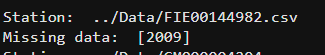
\includegraphics[scale=1]{images/missing.png}}
\caption{Phần dữ liệu bị khuyết}
\end{figure}

\section{Phân tích, đánh giá và kết luận}
Sau khi được tiền xử lý, dữ liệu được trực quan hóa (visualized)thành biểu đồ phân tán nhờ hàm hỗ trợ của module \lstinline{matplotlib}.
\end{document}